\documentclass{config/apuntes}

\title{Caracterización de Redes y Topologías Biológicas}
\author{Sandra Mingo Ramírez}
\date{2024/25}
\acronym{CRRTT}

\usepackage[all]{nowidow}
\usepackage{listing}
\usepackage{color}
\usepackage{tabularx}
\usepackage{multirow}
\usepackage[normalem]{ulem}
\useunder{\uline}{\ul}{}\usepackage{makecell}
\usepackage{amsmath}
\usepackage{array}

\begin{document}

\begin{abstract}
En esta asignatura se estudian los principales tipos de conectividad que se pueden dar en una red biológica. Se describen además cuales puede ser la mejor estrategia de conexión entre los elementos de una red sujetos a una determinada dinámica. También se proporcionan métodos para calcular los principales parámetros topológicos y de rendimiento de una red dada. Además se estudian redes resistentes a una determinada estrategia de ataque o frente a errores en la red.
\end{abstract}

\pagestyle{plain}

\maketitle

\tableofcontents

%40% presentación de proyecto
%60% examen tipo test que resta 33% (nos va a decir lo que entra en el examen)
%Índice de clusterización, camino característico (si no entra uno, entra el otro, pero esos dos seguro)

%18/03 - Carlos Aguirre B322
\chapter{Introducción y descripción de algunas redes reales}
Aunque lo vayamos a utilizar como sinónimos, un grafo y una red no es lo mismo; el grafo es la representación matemática de la red. En una red aleatoria, no hay que medir nada; si una red biológica sale aleatoria, se ha medido mal. Las redes biológicas son todas de mundo pequeño. Además, casi todas son libres de escala. 

\section{Qué es una red}
Una red es un conjunto de elementos (personas, ciudades, proteínas, especies animales, productos químicos, etc) de las cuales algunas están conectadas con otras y otras no. Se puede representar en bolas que se unen con líneas con otras líneas. Las bolitas se denominan como nodos. 

Las redes se estudian con NetworkX y Cytoscape.

\section{Algunos ejemplos de redes y algunas de sus propiedades}
\subsection{World Wide Web}
La World Wide Web es la mayor red para la cual existe información topológica. Los nodos de la red son los documentos, y las ramas son los enlaces (hyperlinks) entre documentos. El tamaño actual de esta red es de más de 1000 millones de nodos. Esta red es dirigida: la página A apunta a la página B, pero sin que la página B apunte a la página A. 
El grupo CAIDA se dedica a analizar la red. Esta red es enorme, pudiendo dibujar solo a un nivel muy alto.

La distribución del grado de las páginas web tiene una distribución libre de escala tanto en los enlaces de salida como en los enlaces de entrada. Esto es una distribución de probabilidad. Por ejemplo, en el queso de Gruyere, los agujeros son de distinto tamaño, los cuales tienen una distribución de tamaño. Se llama libre de escala porque se pueden encontrar diez veces más los agujeros de un tamaño mayor y diez veces menos los agujeros de tamaño pequeño. Así, no hay una escala fija de la distribución (no se puede representar con ninguna escala, ni logarítmica ni nada). Esto con el queso manchego no pasa. Si en la WWW vemos cuántas páginas web tienen 100 enlaces de salida, 10, 1000, etc, y se dibuja en escala logarítmica logarítmica, sale una recta. Esto pasa también con los enlaces de entrada. 

La distancia entre dos páginas de la WWW es pequeña (entre 11 y 16). Los nodos de la WWW están muy clusterizados.

La cola de la derecha parece que rompe la recta. Las redes libres de escala se pueden producir por muchas razones, pero al utilizar un proceso evolutivo en el que cada tiempo se generan nuevos nodos y tienen mayor preferencia para conectarse a otros nodos, e incluso pueden desaparecer algunos nodos antiguos. Esto produce las colas residuales.

\begin{figure}[h]
\centering
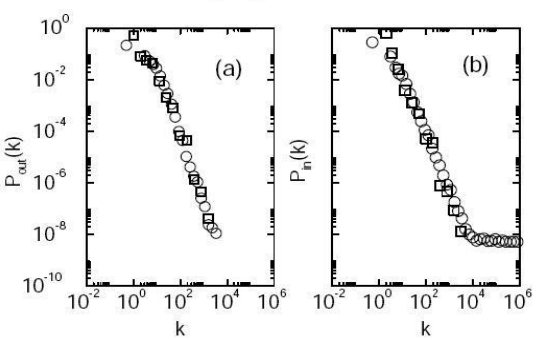
\includegraphics[width = 0.6\textwidth]{figs/www.png}
\end{figure}

Las redes libres de escala son muy resistentes a ataques aleatorios (fallos en la red) en cuanto a la conectividad, por lo que hay una razón evolutiva por la que las redes biológicas son libres de escala. La red regulatoria de P53 está muy estudiada y caracterizada. Uno de los elementos más importantes es MDM5.

\subsection{Internet}
Internet es la red de enlaces físicos entre ordenadores u otros servicios de comunicación. La topología de internet se suele estudiar a dos niveles: Enrutadores y Sistemas autónomos. Los enrutadores son las máquinas que mandan los "paquetes" a otros enrutadores. Hay algoritmos de enrutación que deciden hacia dónde enviar las cosas. Los sistemas autónomos son conjuntos de máquinas que organizan y gestionan otras máquinas.

Para ambos tipos de red (enrutadores y sistemas autónomos) el grado de cada nodo seguía una distribución libre de escala. De nuevo la red está altamente clusterizada (coeficiente de clustering entre 0,18 y 0,3) y los caminos entre nodos son cortos (aproximadamente 9). 

El \textbf{índice de clusterización} es una medida de la probabilidad de que los dos vecinos de un nodo sean vecinos entre sí, favoreciendo la creación de triángulos. Es decir, en redes sociales, que mis amigos también sean amigos entre sí. En biología, si dos proteínas son expresadas por una tercera proteína, las dos mantienen una relación entre sí (aunque puede no pasar). Los vecinos de un mismo nodo tienen una probabilidad alta de ser vecinos entre sí. En una red aleatoria, los vecinos de un nodo dependen de la probabilidad de rama de que esos nodos también sean vecinos entre sí (como cualquier otro).

La métrica de caminos cortos o largos se hace en comparación con el grafo aleatorio con el mismo número de nodos y ramas. En biología, los caminos también suelen ser cortos, y si son largos se puede deber a una enfermedad o patología.

\subsection{Red de actores}
Los nodos son actores, y dos de ellos están conectados si han participado juntos en alguna película. Actualmente, la red consta de unos 450.000 actores.
La distancia media entre actores es 3,65. La red está altamente clusterizada (100 veces más que un grafo aleatorio). La distribución de grados sigue una ley de potencias (libre de escala).

\subsection{Red de colaboración científica}
Los nodos están constituidos por científicos. Dos nodos están conectados si alguna vez publicaron un trabajo en común. La red de nuevo presenta una distribución libre de escala, caminos cortos entre los nodos y una alta clusterización. 

El \textbf{centro de la red} es el nodo que está a una menor distancia promedio del resto de nodos de la red. Este centro lo tiene un científico húngaro llamado Paul Erdös que trabajaba en teoría de grafos. 

Para una red de citaciones científicas, los nodos de la red son artículos científicos. Las ramas son citaciones entre artículos. Se tiene una base de datos de unos 750.000 artículos. Tanto los grados de entrada como los de salida siguen una distribución libre de escala.

\subsection{Red de contactos sexuales}
Los nodos y las ramas tienen una definición obvia. Tiene interés por la difusión de enfermedades (especialmente aquellas de transmisión sexual como el SIDA). Presenta una distribución libre de escala. Se sospecha que los datos de esta red no son totalmente fiables (es defectuosa al tener muchos datos falsos). Entre un 10-15\% es falsa.

Se define como k-core un grafo no dirigido creado a partir de un grafo más grande en el que se crean jerarquías o grupos en el que los nodos están separados por k vértices.

\subsection{Red de llamadas telefónicas}
Los nodos son números de teléfono. Las ramas son llamadas de larga distancia entre nodos. De nuevo la red presenta una distribución libre de escala.

\subsection{Redes lingüísticas}
Los nodos son palabras. Dos nodos están conectados si están juntas en alguna frase y hay solamente una palabra entre ambas. Un estudio realizado en inglés sobre 440.902 palabras presentó una distancia media de 2,62 y un índice de clusterización de 0,43.

Otra red linguística considera de nuevo los nodos como palabras. Dos nodos están conectados si se considera que ambas palabras son sinónimas (de acuerdo con el Merrian Webster Dictionary). El camino medio es de 4,7, el índice de clusterización es de 0,7 y los nodos presentan una distribución libre de escala.

En la red semántica, cada nodo es un objeto o un concepto. Dos nodos se relacionan entre sí, si existe una relación de la forma "es un" o "tiene un" entre ambos nodos. Se ha estudiado poco, pero parece presentar un camino medio corto, alta clusterización y una distribución de nodos libre de escala.

\subsection{Redes eléctricas}
La red eléctrica del Oeste de los Estados Unidos está compuesta por nodos (generadores, transformadores y subestaciones) y ramas (cables físicos entre nodos). La red tiene 4.941 nodos y un grado medio por nodo de 2,41. Esta red se aparta del patrón habitual teniendo una estructura muy jerárquita y en forma de estrella. Esto hace que sea muy frágil y condicionada a cuestiones económicas y políticas. Ocurre de forma similar con las redes de internet. No se utiliza el camino más rápido o corto, si no el camino más barato (como a la hora de buscar vuelos).

\section{Algunos ejemplos de redes biológicas y algunas de sus propiedades}
\subsection{Redes de ecología}
En las redes alimentarias, los nodos de la red son especies, y las ramas relaciones predador-presa entre especies. Las distancias son cortas entre los elementos de la red. En general, son redes con pocos nodos. 

Al ser redes pequeñas es difícil dibujar la distribución del grado de los nodos. Parecen presentar una distribución libre de escala, con un exponente inusualmente pequeño. Esta red es dirigida (aunque pueda haber dobles ramas). 

\subsection{Redes celulares}
Se presentan al estudiar el metabolismo de organismos. Los nodos son sustratos químicos (ATP, ADP, etc), y las ramas presentan reacciones químicas entre los sustratos. Esta red va de arriba a abajo, empezando con unos productos de entrada de la célula y terminando con productos de salida que la célula no puede descomponer más. 

\subsection{Redes neuronales}
Cada nodo es una neurona (biológica o artificial), y las ramas son conexiones sinápticas entre neuronas. La primera red estudiada de este tipo es la del gusano \textit{Caenorhabditis elegans}, del cual se tiene el mapa neuronal completo.

Las redes neuronales artificiales están ahora en auge para las inteligencias artificiales al utilizarse para el aprendizaje profundo.

\subsection{Redes de interacción de proteínas}
Cada nodo es una proteína. Las ramas representan relaciones de expresión entre las proteínas. Una de las redes más importantes es la red p53 de control de crecimiento del cáncer. Un paper muy bueno es \href{https://www.nature.com/articles/35042675}{Surfing the p53 network (DOI 10.1038/35042675)}.

Esta es la red en la que más se trabaja en biología. Se buscan los efectos entre los nodos (aumenta la expresión, inhibe), los componentes clave, los parámetros, etc. 

\subsection{Redes genéticas}
Cada nodo es expresión genética (nucleótidos). Las ramas conectan los nucleótidos que presentan un alto índice de similitud entre ambas. Una vez representada la red, se buscan familias o grupos de genes similares. Hay que diferenciar identidad con similitud (sobre todo con desajuste de fase). Se utiliza programación dinámica para calcular la mayor longitud de subsecuencia idéntica, como por ejemplo con el algoritmo Soldier's Walk. 

Si clusterizamos y obtenemos 2 cluster, cada cluster indica un gen con errores, o dos individuos distintos. Luego hay que interpretar por qué hay ese número de cluster. Normalmente hay muchos clusters que se quieren clasificar, y en cada cluster suele aparecer el mismo gen que se ha mutado. 

Las máquinas de microarrays ahora dan un conjunto de nucleótidos muy grandes, pero antes se obtenían fragmentos que había que unir. Para ello, se debían utilizar algoritmos sobre grafos para calcular cadenas largas a partir de las cadenas cortas, pero ahora ya no se usa por las mejoras tecnológicas. 

%20/03 - Carlos Aguirre
\chapter{Teoría de grafos y métricas}
\section{Introducción a la teoría de grafos}
La teoría de grafos ha sido utilizada recientemente para:
\begin{itemize}
\item Clasificación automática de secuencias de proteínas.
\item Detección de jerarquías de proteínas.
\item Análisis de redes genéticas.
\item Reconstrucción de redes genéticas grandes obtenidas mediante modificación de genes.
\end{itemize}

Un grafo G es un par de conjuntos (V,E) donde $V = \{v_1, v_2, \ldots v_n\}$ es el conjunto de vértices o nodos y $E = \{(v_i, v_j), (v_{i'}, v_{j'}), \ldots \}$ es un conjunto de pares no ordenados de elementos de V y se denomina conjunto de ramas del grafo. 
\marginpar[\footnotesize Pregunta de test: define orden y tamaño, dado un grafo dar el orden y tamaño, etc. ]  \
El número de nodos se denomina \textbf{orden} del grafo, y el número de ramas es el \textbf{tamaño} del grafo. 

\begin{figure}[h]
\centering
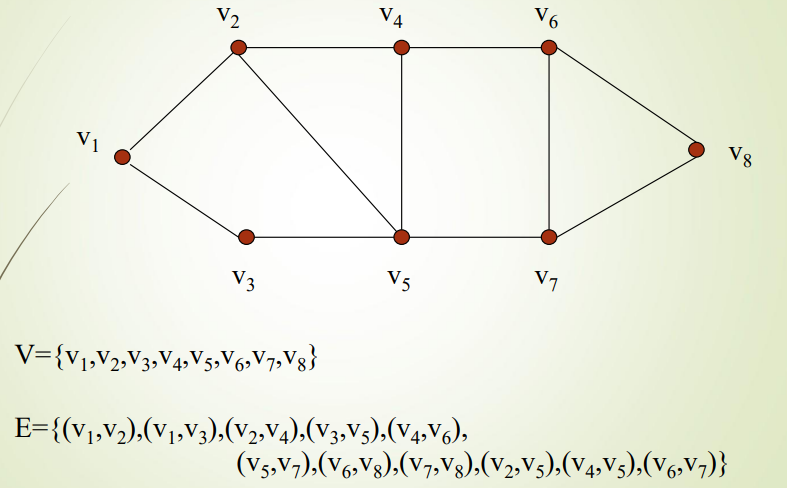
\includegraphics[width = 0.6\textwidth]{figs/grafo.png}
\caption{Ejemplo de grafo de orden 8 y tamaño 11.}
\end{figure}

Para una red de proteínas, cada proteína sería un nodo del grafo, y una rama indicaría interacción entre ambas proteínas. 

Una disposición (layout) es una posible colocación de los nodos y las ramas en un espacio 2D o 3D. Un mismo gráfo puede tener múltiples colocaciones. Ejemplo, consideremos el grafo G=(V,E).

\begin{figure}[h]
\centering
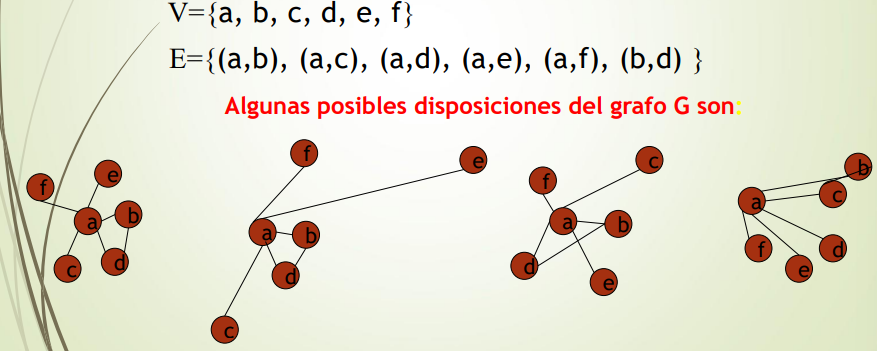
\includegraphics[width = 0.6\textwidth]{figs/layout.png}
\end{figure}

Existen programas de ordenador que nos permiten obtener colocaciones predefinidas (Gephy, Pajek). Cuando no se especifica ninguna colocación, se entiende que los nodos se sitúan aleatoriamente sobre el plano o espacio. Algunos de los tipos más habituales de colocaciones son:
\begin{itemize}
\item Colocaciones regulares
\item Basadas en la física (atracción-repulsión)
\item Basadas en propiedades topológicas (jerarquías, número de vecinos, etc)
\end{itemize}

Un hipergrafo H es un también par de conjuntos (V,E) donde $V=\{v_1, v_2, \ldots v_n\}$ es el conjunto de vértices o nodos y $E=\{(v_{i1}, v_{i2}, \ldots),(v_{i'1},v_{i'2}, \ldots), \ldots\}$ es una familia de
subconjuntos no ordenados de elementos de V. E se denomina conjunto de hiperramas o hiperaristas del hipergrafo. El número de hiperramas $|E|$ se denomina cardinalidad del hipergrafo. El valor $|E|*|V|$ se denomina tamaño o volumen del grafo.
\marginpar[\footnotesize Pregunta examen ]  \
Si tenemos un grafo de n nodos, ¿cuántas parejas podemos tener como máximo? $(n \cdot n-1)/2$ Por tanto, en un grafo con n nodos, ¿cuántas ramas puede tener? Igual, $(n \cdot n-1)/2$

\begin{figure}[h]
\centering
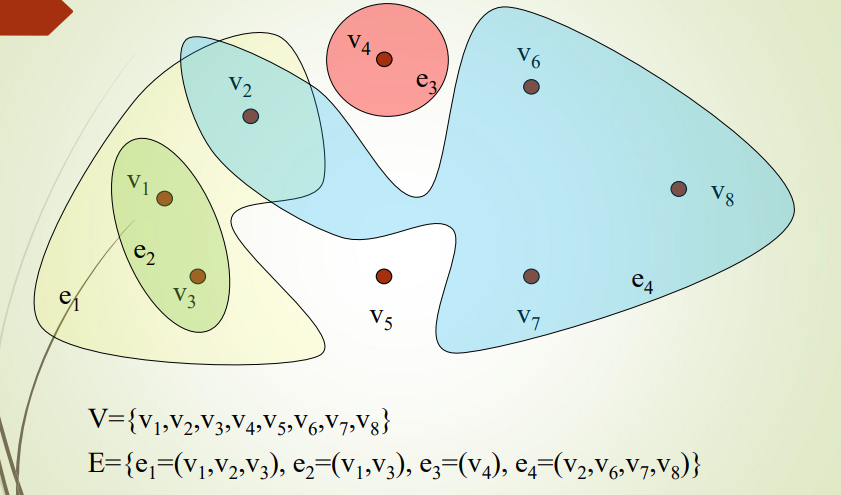
\includegraphics[width = 0.6\textwidth]{figs/hipergrafo.png}
\caption{Ejemplo de hipergrafo de cardinalidad 4 y tamaño 32.}
\end{figure}

Un hipergrafo H se dice que es \textbf{propio} si no es vacío ($V\neq \varnothing$) y no contiene ninguna arista vacía. Un hipergrafo H se dice que tiene \textbf{dominio completo} si todos los nodos están en al menos una arista, en caso contrario se dice que tiene \textbf{dominio parcial}. Si en un hipergrafo todas las hiperramas tienen el mismo número de nodos, entonces se denomina \textbf{hipergrafo k-uniforme}. 

\textit{Ejercicio: Indicar si el hipergrafo del ejemplo anterior es propio, tiene dominio completo y si es k uniforme}. Es propio (el conjunto de vértices tiene 8 elementos y todas las ramas e tienen vértices dentro), es de dominio parcial (v5 no está en ninguna rama) y no es k-uniforme (e1 tiene 3 elementos, e2 tiene 2, e3 tiene 1 y e4 tiene 4).

\section{Bucles y ramas paralelas}
Un bucle es una rama que empieza y termina en el mismo nodo $(v_i, v_i)$. Cuando dos ramas conectan el mismo par de vértices se denominan paralelas. Un grafo con bucles se denomina pseudografo. Un grafo con ramas paralelas pero sin bucles se denomina multigrafos. Un grafo sin bucles ni ramas paralelas se denomina grafo simple.

\begin{figure}[h]
\centering
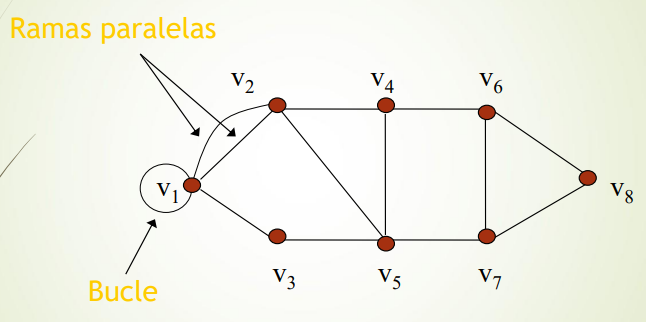
\includegraphics[width = 0.6\textwidth]{figs/bucle-rama-paralela.png}
\end{figure}

%25/03 - Carlos Aguirre
\section{Grafos dirigidos y ponderados}
Se puede considerar que los enlaces entre nodos son dirigidos $(v_i, v_j) = (v_j, v_i)$. Los grafos dirigidos se denominan también \textbf{digrafos}.

\begin{figure}[h]
\centering
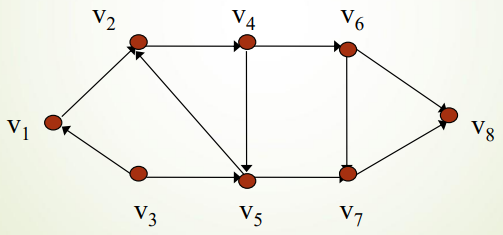
\includegraphics[width = 0.6\textwidth]{figs/grafo-dirigido.png}
\end{figure}

En los grafos ponderados, a cada rama del grafo se le puede asociar un número. El número asociado a cada rama puede indicar entre otras cosas una distancia, una capacidad, un valor temporal, etc.

\begin{figure}[h]
\centering
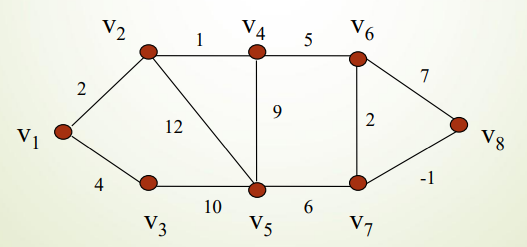
\includegraphics[width = 0.6\textwidth]{figs/grafo-ponderado.png}
\end{figure}

\newpage

Los grafos dirigidos y ponderados poseen ramas dirigidas a las que se asocia un número.

\begin{figure}[h]
\centering
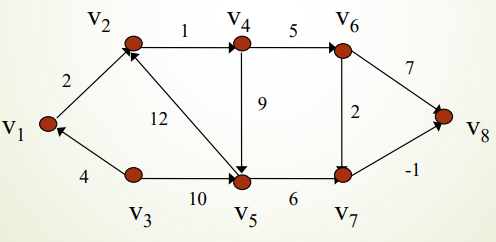
\includegraphics[width = 0.6\textwidth]{figs/grafo-dirigido-ponderado.png}
\end{figure}

\section{Grado de un nodo}
Dos nodos de un grafo son \textbf{vecinos o adyacentes} si existe una rama que los conecta. El \textbf{grado} de un nodo es el número vecinos que tiene dicho nodo. En los grafos dirigidos se calcula el \textbf{grado de entrada} y el \textbf{grado de salida}. En los grafos ponderados, el grado se puede promediar por el número asociado a las ramas. Un grafo se dice que es \textbf{regular} si todos los nodos tienen el mismo grado.

\begin{figure}[h]
\centering
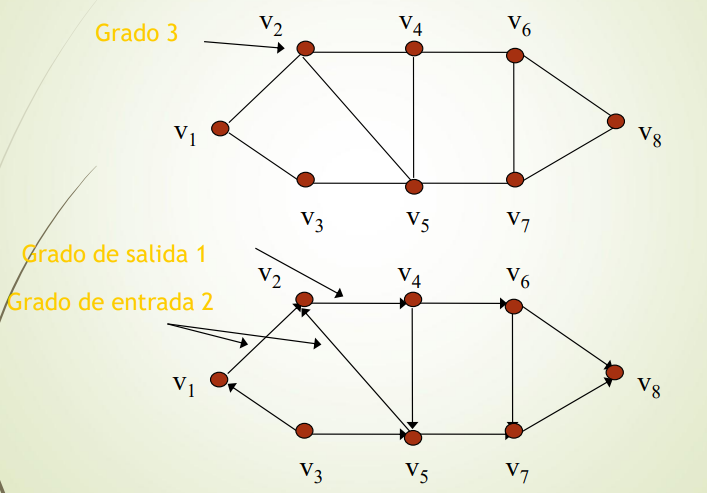
\includegraphics[width = 0.6\textwidth]{figs/grafo-grados.png}
\end{figure}

\section{Subgrafos}
Un grafo G’=(V’,E’) es un subgrafo de un grafo G=(V,E) si V’ es un subconjunto de V y E’ es un subconjunto de E. En otras palabras, un subgrafo es un trozo de un grafo más grande. 

\begin{figure}[h]
\centering
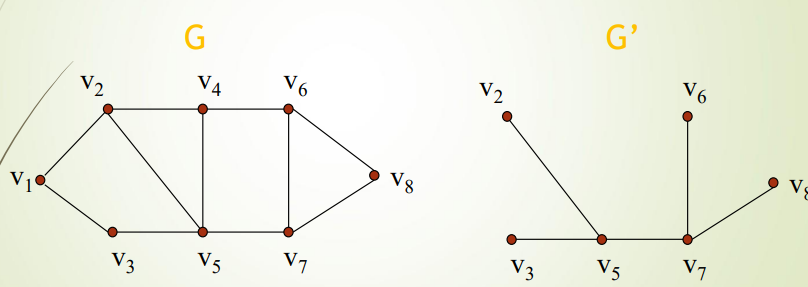
\includegraphics[width = 0.6\textwidth]{figs/subgrafo.png}
\end{figure}

Un subgrafo G’=(V’,E’) de un grafo G=(V,E) se dice que es \textbf{abarcador} si V=V’, es decir, si están todos los nodos, pero faltan algunas ramas.

Un grafo es un subgrafo de sí mismo. Además, un grafo vacío es un subgrafo de cualquier grafo.

\section{Paseos, caminos, circuitos y ciclos}
Un \textbf{paseo} de un nodo u a un nodo v es una secuencia de vértices $\{v_0, v_1, \ldots, v_k\}$ con $v_1 = u v_k = v$ y $(v_{i-1}, v_i)$ rama del grafo. El número de ramas del paseo es su \textbf{longitud}. Un paseo en el cual no se repiten ramas se denomina \textbf{rastro}. Un paseo en el cual todos los vértices $\{v_0, v_1, \ldots, v_k\}$ son distintos se denomina \textbf{camino}. 
Un camino siempre debe ser un rastro y un paseo. Si algo no es rastro, no puede ser camino, y si no es paseo, no puede ser ni rastro ni camino. Cada uno es cada vez más restrictivo.

Entre dos nodos, puede haber varios caminos posibles. Un \textbf{camino mínimo} entre dos nodos es aquel de menor longitud de entre todos los posibles caminos entre ambos nodos. La \textbf{distancia} entre dos nodos del grafo se define como la longitud de cualquier camino mínimo que los una.

\begin{figure}[h]
\centering
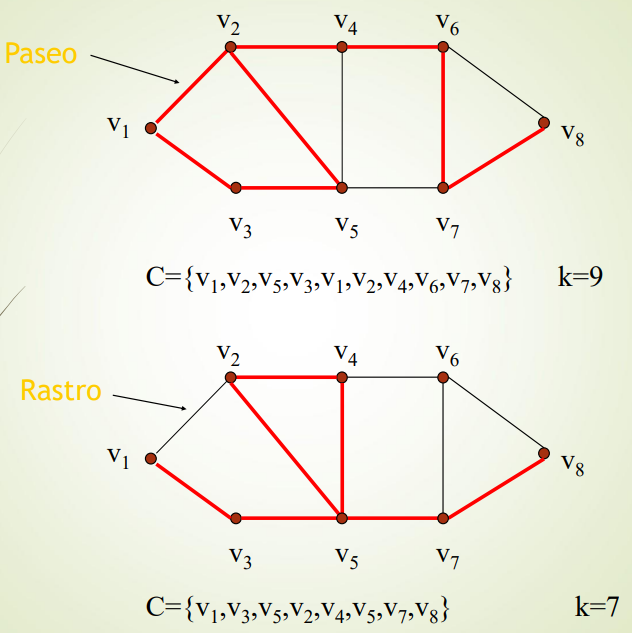
\includegraphics[width = 0.5\textwidth]{figs/paseo-rastro.png}
\end{figure}

\begin{figure}[h]
\centering
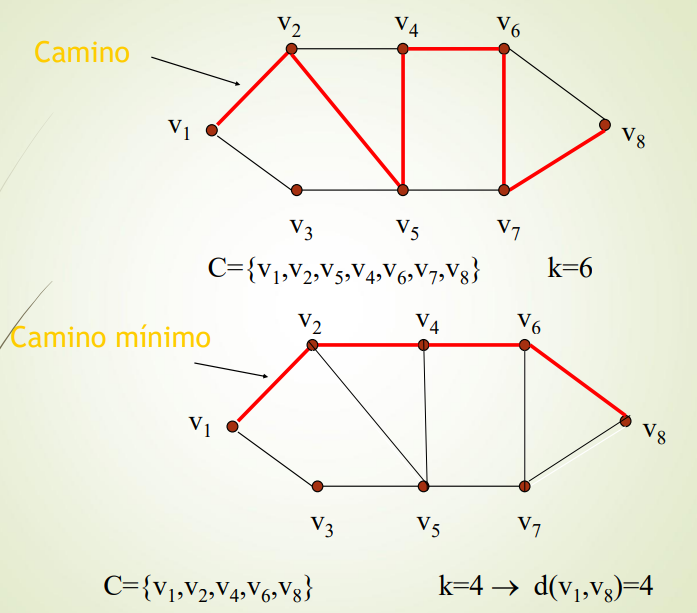
\includegraphics[width = 0.5\textwidth]{figs/camino-minimo.png}
\end{figure}

Un \textbf{paseo cerrado} es un paseo $\{v_0, v_1, \ldots, v_k\}$ tal que $v_0 = v_k$. Un paseo cerrado en el que no se repiten ramas es un \textbf{circuito}. Un \textbf{ciclo} es un circuito en el que no se repiten vértices. Los ciclos son importantes, porque las redes biológicas tienen ciclos (que suelen ser largos), pero en las redes aleatorias no aparecen ciclos, o éstos son muy pequeños.

\begin{figure}[h]
\centering
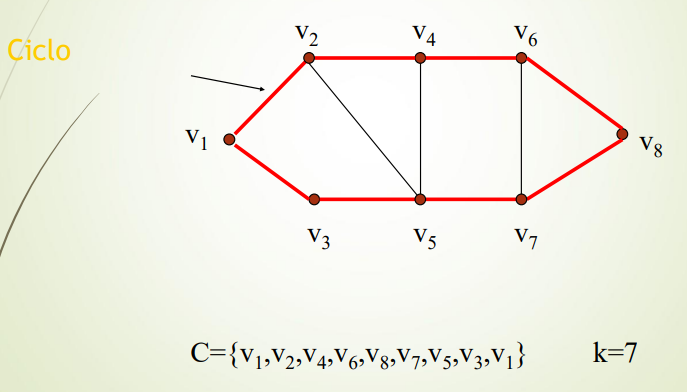
\includegraphics[width = 0.5\textwidth]{figs/ciclo.png}
\end{figure}

El nodo con menor distancia entre los demás es muy importante, denominándose como \textbf{centro del grafo}.

Para un grafo con excesivos nodos, los caminos mínimos y las distancias se calculan con un algoritmo. Si el grafo es no ponderado, se utiliza el algoritmo búsqueda en anchura, mientras que si es ponderado, utiliza Dijkstra.

\section{Medidas de centralidad, betweeness y closeness}
\marginpar[\footnotesize Pregunta examen: Betweeness/Closeness/Farness se define como... ]  \
Dado un nodo $v_i$ se define su \textbf{betweeness} $C_B (v_i)$ como la fracción de caminos mínimos que hay entre el resto de nodos del grafo y que pasan por el nodo $v_i$. Es decir, se hacen parejas de todos los nodos del grafo excluyendo el nodo de interés, y se calculan los caminos mínimos. Algunos pasarán por el nodo de interés, que son los que nos quedamos. Con eso se evalúa el cociente (los que pasan por ese nodo entre todos), que será el betweeness (un valor entre 0 y 1).
La centralidad de un nodo es muy costosa de calcular, usualmente se emplean algoritmos aproximados. 

Dado un nodo $v_i$ se define su \textbf{lejanía o farness} $C_F (v_i)$ como la suma de las distancias de $v_i$ al resto de nodos del grafo. 

Dado un nodo $v_i$ se define su \textbf{cercanía o closeness} $C_C (v_i)$ como la inversa de su lejanía $C_C (v_i) = 1/C_F (v_i)$.

\begin{figure}[h]
\centering
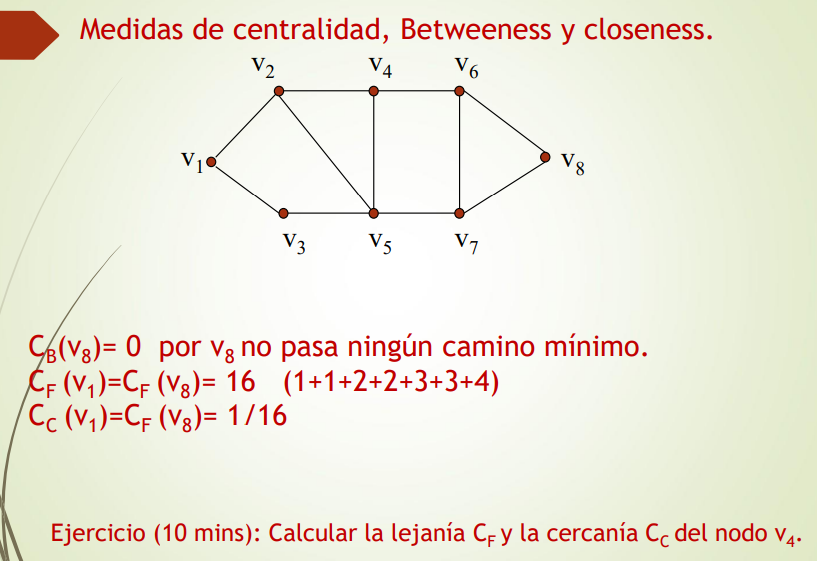
\includegraphics[width = 0.5\textwidth]{figs/medidas-centralidad.png}
\caption{Respuesta al ejercicio: Cogiendo v4, la lejanía será 2+1+2+1+1+2+2 = 11, y la cercanía 1/11.}
\end{figure}

La cercanía y lejanía tiene un problema: su valor numérico depende del orden del grafo. Por tanto, sirve para comparar dentro del mismo grafo, pero no entre grafos. 
\marginpar[\footnotesize Pregunta examen: Calcular camino característico ] \
Para eso, habría que normalizar dividiendo por el número total de nodos. A esto se le conoce como \textbf{camino característico}.

\section{Conexidad}
Un grafo es \textbf{conexo} si para cada par de nodos del grafo existe al menos un camino que los une. En otras palabras, que no esté separado en distintos trozos. 

\begin{figure}[h]
\centering
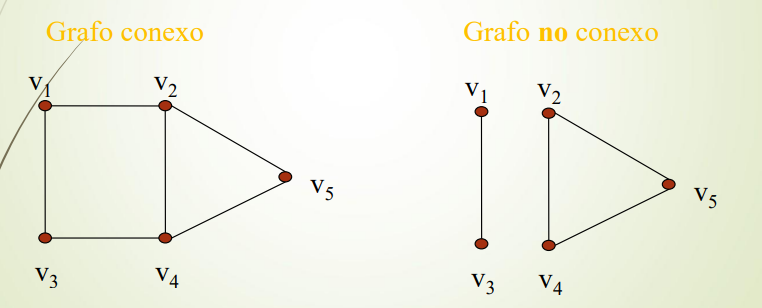
\includegraphics[width = 0.6\textwidth]{figs/conexidad.png}
\end{figure}

Hay un algoritmo muy rápido y eficiente que calcula si un grafo es conexo o no. 

Una \textbf{componente conexa} de un grafo es cada uno de los subgrafos
maximales conexos. Esto quiere decir que el subgrafo no puede ser más grande, que no se le puede añadir más nodos.

\begin{figure}[h]
\centering
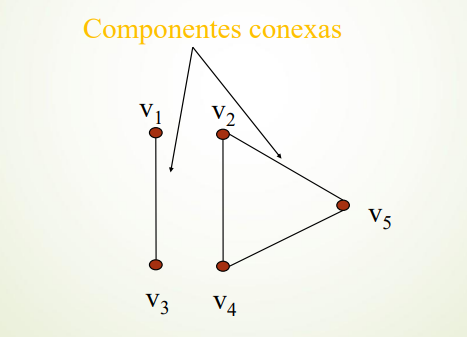
\includegraphics[width = 0.5\textwidth]{figs/componentes-conexas.png}
\end{figure}

Un \textbf{punto de articulación} es un nodo que desconecta un grafo conexo. Un \textbf{corte} es un conjunto de ramas que desconecta un grafo conexo. Si un corte esta compuesto por una única rama, se denomina \textbf{puente}. Un \textbf{corte mínimo} de un grafo es el mínimo número de ramas que al ser eliminadas desconectan el grafo.

El algoritmo CLICK (CLuster Identification via Connectivity Kernels) calcula una aproximación al corte mínimo. Esto lo hacían cogiendo los dos nodos más lejanos. Los puentes suelen ser muy malos para la conexidad de los grafos. 

\begin{figure}[h]
\centering
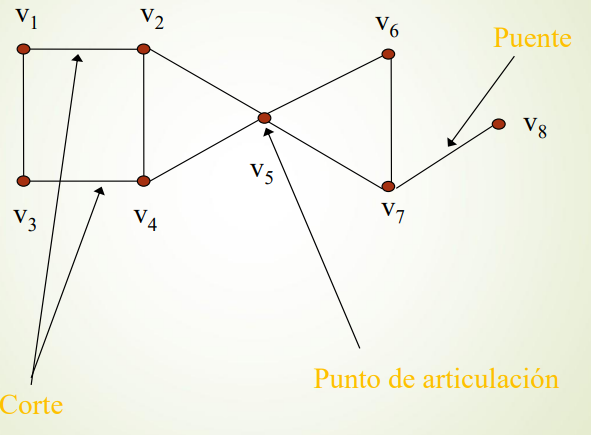
\includegraphics[width = 0.5\textwidth]{figs/conexidad2.png}
\end{figure}

La máxima distancia entre cualquier par de nodos se denomina como diámetro.

El corte mínimo entre dos nodos es siempre mayor que el corte mínimo de todo el grafo.  

\section{Bosques y árboles}
Un grafo sin ciclos (acíclico) se denomina bosque. Un árbol es un grafo acíclico conexo. Cada componente conexa de un bosque es un árbol.

\begin{figure}[h]
\centering
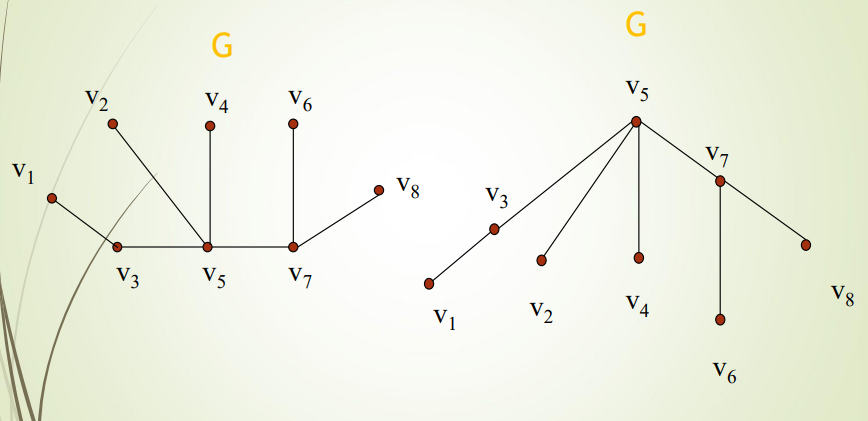
\includegraphics[width = 0.6\textwidth]{figs/arbol-bosque.png}
\end{figure}

Un subgrafo abarcador acíclico de un grafo G se denomina un \textbf{bosque abarcador}. Un subgrafo abarcador conexo acíclico de un grafo G se denomina un \textbf{árbol abarcador}.

\begin{figure}[h]
\centering
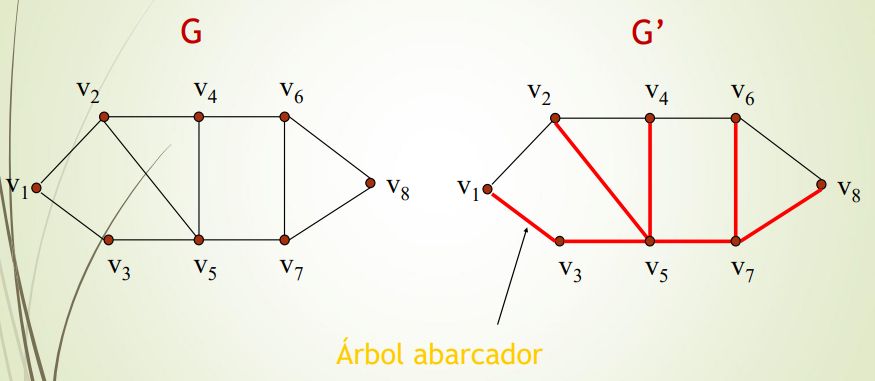
\includegraphics[width = 0.6\textwidth]{figs/arbol-abarcador.png}
\end{figure}

%27/03 - Carlos Aguirre
\section{Grafos bipartitos}
Un grafo se dice que es bipartito si:
\begin{itemize}
\item El conjunto de vértices V se puede romper en dos subconjuntos disjuntos V1 y V2.
\item El vértice inicial de cada rama de E pertenece a V1 y el vértice final a V2
\end{itemize}

Ejercicio: el grafo anterior (el del árbol abarcador), ¿es bipartito? No, porque no es posible realizar la partición. Si V1 pertenece al conjunto 1, V2 y V3 deben estar en el conjunto 2, por lo que V4 y V5 tienen que estar en V1, pero esto no es posible porque están conectados entre sí. La condición necesaria para que un grafo sea bipartito es que no tenga triángulos. Pero esto no es suficiente; se puede construir un grafo sin triángulos, pero que tampoco sea bipartito. Si cogemos solo el cuadrado V4-V7, sí se podría generar un grafo bipartito: V4 y V7 en un conjunto y V5 y V6 en otro. 

\section{Representación de grafos}
Hay dos formas estándar de representar un grafo en un ordenador:
\begin{itemize}
\item \textbf{Matriz de adyacencia}: consume mucha memoria, pero es fácil de añadir o eliminar ramas. Es fácil saber si existe una rama, pero es lento enumerar los vecinos de un nodo. Se pueden calcular los autovalores y autovectores.
\item \textbf{Lista de adyacencia}: tiene un consumo limitado de memoria, pero es costoso añadir o eliminar ramas. También es costoso saber si existe una rama, pero rápido enumerar los vecinos de un nodo.
\end{itemize}

\section{Métricas sobre grafos}
Los grafos se clasifican en función de unas determinadas métricas topológicas. Las métricas más empleadas son:
\begin{itemize}
\item Tamaño |E| y orden |V|
\item Dispersión: $\frac{2 |E|}{|V| (|V| - 1)}$ para un grafo no dirigido y $\frac{|E|}{|V| (|V| - 1)}$ para un grafo dirigido. Si el coeficiente es pequeño (0), el grafo es disperso, si es cercano a 1, es denso. En redes biológicas, los grafos suelen ser dispersos.
\item Distribución del grado de los nodos: división del grado de todos los nodos entre el número de nodos. El resultado es una distribución de probabilidad. En un grafo aleatorio, la distribución es de Poisson (como la gaussiana, pero sin valores negativos). En las redes biológicas, la distribución no será de Poisson, por lo que este será el primer test que se haga a los datos. 
\item Grado medio (<k>)
\item Coeficiente de agrupamiento
\item Camino característico (L)
\end{itemize}

\subsection{Coeficiente de agrupamiento}




\end{document}
